\documentclass[11pt]{article}
\usepackage{amssymb}
\usepackage[english]{babel}
\usepackage{fullpage}
\usepackage{graphicx}
\usepackage{pythonhighlight}

\def\titre{}
\def\auteur{}
\def\courriel{}
\makeatletter

\title{}

\author{}

\date{}

\begin{document}
\maketitle

\section{Infrastructure setup}

\paragraph{Instances}\mbox{}\\
The instances created will be five M4.large instances (two 2.4 GHz Intel Xeon E5-2676 vCPUs, 8 GiB memory, moderate network performance and 450 Mbps) and five T2.large instances (two Intel vCPUs, 8 GiB of memory and low to moderate network performance). However, due to account restrictions, we can only deploy a total of nine instances, so the second group will only have four. Each instance will allow SSH, HTTP and HTTPS traffic from 0.0.0.0/0, meaning the whole internet. The operating system is ubuntu and the image used is ami-08c40ec9ead489470. The availability zone will be us-east-1. Flask will be deployed on each instance at IP address 0.0.0.0 port 80.

\paragraph{Target groups:}\mbox{}\\
The first target group will include all five M4.large instances, while the second one will be four T2.large instances. The targets will receive traffic on port 80. IPv4 will be used with the HTTP protocol.

\paragraph{Elastic load balancer:}\mbox{}\\
The elastic load balancer will be an internet facing application load balancer (requests can be routed based on their contents such as the URL path). IPv4 is used. Its security group allows it to send and receive traffic from anywhere on the internet (TCP to and from 0.0.0.0/0). Two subnet IDs are specified (us-east-1a and us-east-1b).

\paragraph{Listener}\mbox{}\\
The listener listens on port 80 and will send requests to one of the two target groups that are attached to it. The protocol is HTTP, and both target groups are given equal weight. The URL path for the first target group is /cluster1 and the URL path for the second target group is /cluster2. The paths are specified in the value

\begin{python}
    Conditions=[
        {
            'Field': 'path-pattern',
            'PathPatternConfig': {
                'Values': [
                    path
                ]
            },
        },
    ],
\end{python}
The diagram of the setup is as follows:

\begin{figure}
    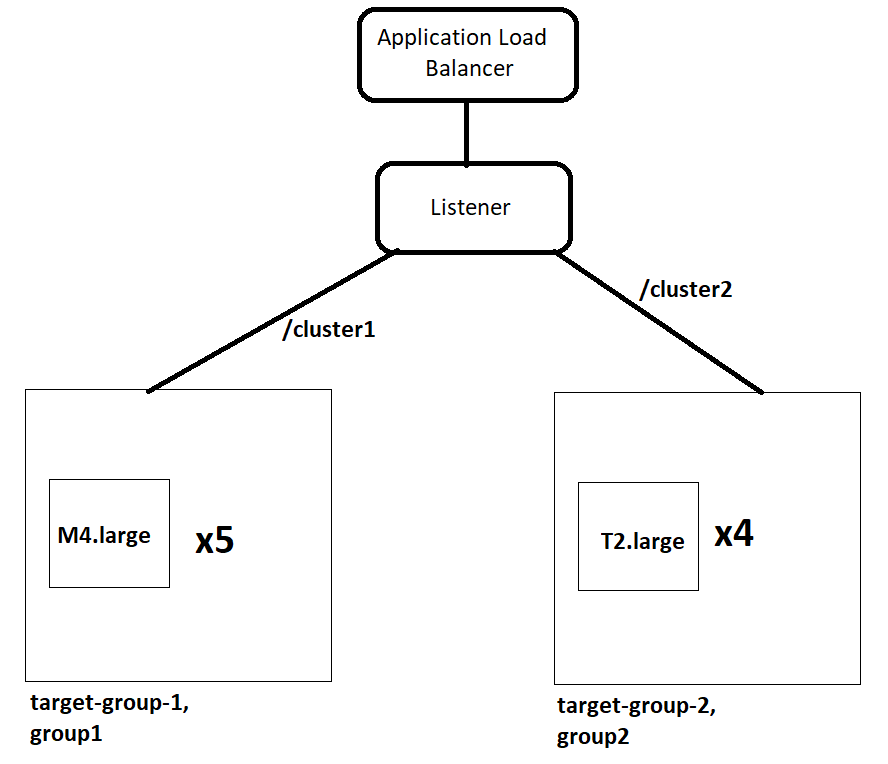
\includegraphics[width=\linewidth]{cluster.png}
    \caption{Application load balancer with 2 clusters and a forward listener}
    \label{fig:setup}
\end{figure}


\end{document}